\documentclass[12pt]{article}

\usepackage{algorithm}
\usepackage{float}
\usepackage{algpseudocode}
\usepackage{algorithmicx}
\usepackage{algpseudocode}
\usepackage{answers}
\usepackage{authblk}
\usepackage{ctex}
\usepackage{setspace}
\usepackage{graphicx}
\usepackage{enumitem}
\usepackage{multicol}
\usepackage{mathrsfs}
\usepackage[margin=1in]{geometry} 
\usepackage{amsmath,amsfonts,amsthm,amssymb}
\usepackage{mathtools}
\usepackage{multirow}
\usepackage{xcolor}
\usepackage{makecell}
\usepackage{url}
\usepackage{fontspec}
\usepackage{hyperref}
\usepackage[bottom]{footmisc}
\usepackage{hologo}
\usepackage{wallpaper}
\usepackage{makecell}
\usepackage{listings, lstautogobble}
\usepackage{color}

\definecolor{mygreen}{rgb}{0,0.6,0}
\definecolor{mygray}{rgb}{0.5,0.5,0.5}
\definecolor{mymauve}{rgb}{0.58,0,0.82}

\NewDocumentCommand{\code}{v}{
	\texttt{\textcolor{blue}{#1}}
}

\CenterWallPaper{.50}{img/zju_logo.png}
\hypersetup{
    colorlinks=true,
    linkcolor=blue,
	urlcolor=magenta,
	citecolor=red      
}

\newcommand{\ver}{\textmd{Version} 3.0} % Version number.

\newcommand{\mat}[1]{\boldsymbol{#1}}
\newcommand{\spc}[1]{\textit{#1}}
\renewcommand{\vec}[1]{\boldsymbol{#1}}

\newcommand{\N}{\mathbb{Z}^+}
\newcommand{\Z}{\mathbb{Z}}
\newcommand{\Q}{\mathbb{Q}}
\newcommand{\Qp}{\mathbb{Q}^+}
\renewcommand{\C}{\mathbb{C}}
\newcommand{\R}{\mathbb{R}}
\newcommand{\F}{\textit{F}}
\newcommand{\T}{\textit{T}}
\renewcommand{\P}{\textit{P}}
\newcommand{\J}[1]{\textit{J}_{\mat{#1}}}
\newcommand{\V}{\spc{V}}
\newcommand{\E}{\spc{E}}
\renewcommand{\L}{\mathcal{L}}

\newcommand{\inv}{^{\mathsf{-1}}}
\newcommand{\herm}{^{\mathsf{H}}}
\newcommand{\PI}{\displaystyle \prod}

\newcommand{\adj}[1]{\operatorname{adj}(\mat{#1})}
\DeclareMathOperator{\spn}{span}
\DeclareMathOperator{\rnk}{rank}
\DeclareMathOperator{\nul}{nullity}
\DeclareMathOperator{\Ker}{N} % Capital, since \ker is already defined.
\DeclareMathOperator{\lker}{Lker}
\DeclareMathOperator{\im}{Im}
\DeclareMathOperator{\cs}{CS}
\DeclareMathOperator{\rs}{RS}
\DeclareMathOperator{\tr}{tr}
\DeclareMathOperator{\cof}{cof}
\DeclareMathOperator{\am}{am}
\DeclareMathOperator{\gm}{gm}
\DeclareMathOperator{\len}{Length}
\DeclareMathOperator{\num}{Number}
\newcommand{\ii}{{i\mkern1mu}}
\newcommand{\dotp}[2]{<#1, #2>}
\newcommand{\proj}[2]{\operatorname{proj}_{#1}\vec{#2}}
\newcommand{\Mod}[1]{\ (\mathrm{mod}\ #1)}
\DeclarePairedDelimiter{\ceil}{\lceil}{\rceil}
\DeclarePairedDelimiter{\floor}{\lfloor}{\rfloor}

\newcommand{\tnr}{\fontspec{Times New Roman}}
\newcommand{\con}{\fontspec{Consolas}}
 
\newenvironment{theorem}[2][Theorem]{\begin{trivlist}
\item[\hskip \labelsep {\bfseries #1}\hskip \labelsep {\bfseries #2}]}{\end{trivlist}}

\renewcommand{\contentsname}{Table of Contents}
\renewcommand{\refname}{References}
\renewcommand{\tablename}{Table}
\renewcommand{\figurename}{Figure}

\begin{document}

\title{\Huge{\textbf{計算機組織}} \\
	\LARGE{\textbf{Computer Architecture}}
}
\newcommand*{\affaddr}[1]{#1}
\newcommand*{\affmark}[1][*]{\textsuperscript{#1}}
\author{
	TZU-CHUN HSU\affmark[1] \\
	\affmark[1]\href{mailto:vm3y3rmp40719@gmail.com}{vm3y3rmp40719@gmail.com} \\
	\affaddr{\affmark[1]Department of Computer Science, Zhejiang University
	}
}

\date{\mbox{}\vfill\today\\ \ver}

\maketitle
\pagebreak

\addcontentsline{toc}{section}{Disclaimer}
\begin{center}
    \Huge{\texttt{Disclaimer}}\\
\end{center}

本文「演算法」為台灣研究所考試入學的「演算法」考科使用,內容主要參考洪捷先生的演算法參考書\cite{1},以及wjungle網友在PTT論壇上提供的演算法筆記\cite{2}。 \\
本文作者為\textsc{TZU-CHUN HSU},本文及其\hologo{LaTeX}相關程式碼採用\textbf{MIT協議},更多內容請訪問作者之\textsc{GitHub}分頁\href{https://github.com/Oscarshu0719}{Oscarshu0719}。 \\~\\

\con
MIT License

Copyright (c) 2020 TZU-CHUN HSU

Permission is hereby granted, free of charge, to any person obtaining a copy
of this software and associated documentation files (the "Software"), to deal
in the Software without restriction, including without limitation the rights
to use, copy, modify, merge, publish, distribute, sublicense, and/or sell
copies of the Software, and to permit persons to whom the Software is
furnished to do so, subject to the following conditions:

The above copyright notice and this permission notice shall be included in all
copies or substantial portions of the Software.

THE SOFTWARE IS PROVIDED "AS IS", WITHOUT WARRANTY OF ANY KIND, EXPRESS OR
IMPLIED, INCLUDING BUT NOT LIMITED TO THE WARRANTIES OF MERCHANTABILITY,
FITNESS FOR A PARTICULAR PURPOSE AND NONINFRINGEMENT. IN NO EVENT SHALL THE
AUTHORS OR COPYRIGHT HOLDERS BE LIABLE FOR ANY CLAIM, DAMAGES OR OTHER
LIABILITY, WHETHER IN AN ACTION OF CONTRACT, TORT OR OTHERWISE, ARISING FROM,
OUT OF OR IN CONNECTION WITH THE SOFTWARE OR THE USE OR OTHER DEALINGS IN THE
SOFTWARE.

\tnr
\pagebreak

\section{Overview}

\begin{enumerate}
    \item 本文頁碼標記依照實體書\cite{1}\cite{2}的頁碼。
    \item TKB筆記\cite{3}章節頁碼:
    \begin{table}[H]
        \centering
        \begin{tabular}{|c|c|}
            \hline
            Chapter & Page No. \\
            \Xhline{2\arrayrulewidth}
            1 & 1 \\
            \hline
            2 & 27 \\
            \hline
            3 & 81 \\
            \hline
            4 & 101 \\
            \hline
            5 & 119 \\
            \hline
            6 & 165 \\
            \hline
            7 & 221 \\
            \hline
            8 & 238 \\
            \hline
        \end{tabular}
    \end{table}
    \item 常考:(參考TKB筆記\cite{3}中頁碼)
    \begin{enumerate}
        \item 19 
        \item 59
        \item 84
        \item 92
        \item 141
        \item 170
        \item 200
    \end{enumerate}
    \item 省略第一章重點十四,第二章重點五、六、十,第六章重點十四,第七章只看重點一到四及十,第八章重點五一致性協定範例。
\end{enumerate}

\pagebreak
\begingroup
\section{Summary}
\begin{enumerate}
\let\clearpage\relax
\item \begin{theorem}{(1.6)} $\phi$為任何集合的子集。
\end{theorem}

\item \begin{theorem}{(1.16)} \begin{subequations}
    \begin{align}
        \P(A \cup B) & \neq \P(A) \cup \P(B) \\
        \P(A \cap B) & = \P(A) \cap \P(B)
    \end{align}
    \end{subequations}
\end{theorem}

\item \begin{theorem}{(1.55)} 若$a, b, c \in \N$,則$ax + by = c$有整數解$\iff$$\gcd(a, b) | c$。
\end{theorem}

\item \begin{theorem}{(1-42)1.92} $2^{mn} \Mod{2^m - 1} = 1$。
\end{theorem}

\item \begin{theorem}{(1.58, 1.60)} (質數)
    \begin{itemize}
        \item 若$a \in \Z, n \in \N$,且$\gcd(a, n) = 1$,則$a^{-1} \Mod{n}$存在。
        \item 若$p$為質數,$a \in \Z$,則$a^{-1} \equiv a \Mod{p}$即$a^2 \equiv 1 \Mod{p}$$\iff$$a \equiv \pm 1 \Mod{p}$。
    \end{itemize}
\end{theorem}

\item \begin{theorem}{(1.62)} 若$a, b, c, n \in \Z$,若$\gcd(c, n) = 1$,則$ac \equiv bc \Mod{n}$$\iff$$a \equiv b \Mod{n}$。
\end{theorem}

\item \begin{theorem}{(1.61, 1.62)} (質數)
    \begin{itemize}
        \item Wilson's theorem:
        若$p$為質數,則
        \begin{equation}
            (p - 1)! \equiv -1 \Mod{p}
        \end{equation}
        \item Fermat's little theorem:
        若$p$為質數,$m \in Z$,且$\gcd(m, p) = 1$,則
        \begin{equation}
            m^{p - 1} \equiv 1 \Mod{p}
        \end{equation}
    \end{itemize}
\end{theorem}

\item \begin{theorem}{(1.64, 1.65, 1.66)} (質數)
    \begin{itemize}
        \item 若$n \in \N$,則Euler $\phi$-函數$\phi(n)$為$\{1, 2, \ \cdots, n - 1\}$中與$n$互質的元素個數,又稱Euler's totient function。
        \item 若$n = p_1^{e_1}p_2^{e_2}\cdots p_k^{e_k}$為$n$的質因數分解,則$\phi(n) = n\PI_{j = 1}^{k}(1 - \frac{1}{p_j})$。
        \item 若$p \in \N$,則$\phi(p) = p - 1$$\iff$$p$為質數。
        \item 若$m \in \Z, n \in \N$,且$\gcd(m, n) = 1$,則$m^{\phi(n)} \equiv 1 \Mod{n}$。
        \item 若$p$為質數,$m \in Z$,且$\gcd(m, p) = 1$,則$m^{-1} \equiv m^{p - 2} \Mod{p}$
    \end{itemize}
\end{theorem}

\item \begin{theorem}{(1.66)} 中國餘數定理(Chinese Remainder Theorem,CRT)中,模的數之間必須互質。
\end{theorem}

\item \begin{theorem}{(1.71)} RSA公鑰密碼系統(RSA public key cryptosystem):\begin{itemize}
        \item 訊息:$M$。
        \item 加密鑰(encryption key):\begin{equation}
            n = pq, \ e
        \end{equation}
        其中$p, q$為質數,且$\gcd(e, \phi(n)) = 1, \ \phi(n) = (p - 1)(q - 1)$。
        \item 加密訊息:\begin{equation}
            C = M^e \Mod{n}
        \end{equation}
        \item 解密鑰(decryption key):\begin{equation}
            d \equiv e^{-1} \Mod{\phi(n)}
        \end{equation}
        \item 解密訊息:\begin{equation}
            C^d \equiv M \Mod{n}
        \end{equation}
    \end{itemize}
\end{theorem}

\item \begin{theorem}{(2.51)} (可逆)若$\mat{A}$為可逆上三角矩陣,則$\adj{A}$和$\mat{A}\inv$也是上三角矩陣。
\end{theorem}

\item \begin{theorem}{((2-45)2.92)} (可逆,方陣)若$\mat{A}, \mat{B} \in \F^{n \times n}$為可逆方陣,則$\adj{\mat{AB}} = \adj{\mat{B}}\adj{\mat{A}}$。
\end{theorem}


\begin{theorem}{(60, 61)} Process life cycles (Figure \ref{img:process_lifecycles}): \begin{itemize}
        \item State:\begin{itemize}
            \item New (Created):Process is created and PCB is allocated in kernel, but memory space is NOT allocated.
            \item Ready:Process is allocated memory space.
        \end{itemize}
        \item Transition:\begin{itemize}
            \item Admitted:Process is allocated memory space. In batch system, use long-term scheduler to decide which process to load into memory. In time-sharing and real-time systems, do NOT use long-term scheduler.
            \item Dispatch:Short-term (CPU) scheduler decides which process to get CPU allocation and allocates CPU to execute.
            \item Interrupt (Time-out):e.g. time-out interrupt.
        \end{itemize}
        \item Zombie state:Process is finished, but the parent process have NOT collected results of the children processes, or parent process have NOT executed wait() system call. Resources are released, but PCB have NOT been deleted, until parent process collects the results, then kernel delete PCB.
    \end{itemize}
\end{theorem}

\begin{figure}[H]
    \centering
    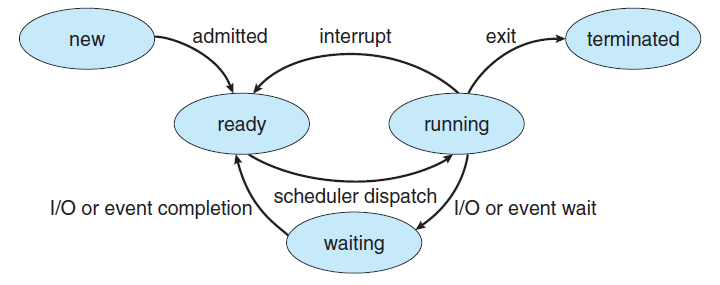
\includegraphics[scale=0.8]{img/process_lifecycles.png}
    \caption{Process life cycles.}
    \label{img:process_lifecycles}
\end{figure}

\begin{theorem}{(67)} Scheduler:\begin{itemize}
        \item Long-term (Job) scheduler:通常batch system採用,time-sharing與real-time systems不採用,從job queue中選jobs載入memory。執行頻率最低,可以調控multiprogramming degree與CPU-bound與I/O-bound jobs的比例。
        \item Short-term (CPU, process) scheduler:從ready queue選擇一個process分派給CPU執行。所有系統都需要,執行頻率最高,\textbf{無法}調控multiprogramming degree與CPU-bound與I/O-bound jobs的比例。
        \item Medium-term scheduler:Memory space不足且有其他processes需要更多memory時執行,選擇Blocked或lower priority process swap out to disk。Time-sharing system採用,batch和real-time systems不採用,可以調控multiprogramming degree與CPU-bound與I/O-bound jobs的比例。
    \end{itemize}
\end{theorem}

\begin{theorem}{(69, 70)} \quad\quad \begin{itemize}
        \item Context switch:\begin{itemize}
            \item 執行期間無法執行process,主要取決於硬體因素。
            \item 降低負擔:\begin{itemize}
                \item 提供Multiple registers set:每個process有自己的registers set,只需要切換pointer就能context switch。
                \item 使用Multi-threading。
            \end{itemize}
        \end{itemize}
        \item Dispatcher:\begin{itemize}
            \item 將CPU真正分配給CPU scheduler選擇的process。
            \item Context switch.
            \item Switch mode to user mode.
            \item Jump to execution entry of process.
        \end{itemize}
    \end{itemize}
\end{theorem}

\begin{theorem}{(63)} Process control operation: \begin{itemize}
        \item \code{fork()}:\begin{itemize}
            \item child process有與parent process不同的memory space,而起始code section和data section皆來自parent process的複製。
            \item 失敗:回傳負值;成功:回傳$0$給child process,$> 0$值即child process PID給parent process。
        \end{itemize}
        \item \code{wait()}:若child process已終止,帶parent process還沒執行$wait()$,但kernel含不能清除child process PCB,直到parent process收集完child process info,此段期間稱zombie。
        \item \code{execlp(dir, filename, args)}:載入特定工作執行,memory content不再是parent process的複製,沒有參數填\code{NULL},e.g. \code{execlp("/bin/ls", "ls", NULL)}。
    \end{itemize}
\end{theorem}

\begin{theorem}{(70)} 評估scheduling performance: \begin{itemize}
        \item Waiting time:Process在\textbf{ready queue}的時間。
        \item Turnaround:Process\textbf{進入系統到完成工作}的時間。
        \item Response time:User輸入到系統產生第一個回應的時間。
    \end{itemize}
\end{theorem}

\begin{theorem}{(75)} Starvation:\begin{itemize}
        \item 有機會完成但是機會很小。
        \item 通過Aging解決:當process在系統中時間增加,逐漸提升process的prioirty。但是soft real-time systems不能使用Aging,因為會違反定義。
    \end{itemize}
\end{theorem}

\begin{theorem}{(71, 72, 75, 76, 77, 78)} Scheduling algorithms: \begin{itemize}
        \item FCFS (First-come-first-serve):可能遭遇Convoy effect,即許多processes都在等待一個需要很長CPU time的process完成工作。
        \item SJF (Shortest-Job-First):\begin{itemize}
            \item Preemptive SJF又稱SRTF (Shortest-Remaining Time First)。
            \item 效益最佳(包含SRTF),即平均等待時間最短。
            \item 對long-burst time job,可能有starvation。
            \item 不適合用在CPU (short-term) scheduling,因為不知道process的精確next CPU burst time,短時間也難以精準預估。
            \item Long-term job可能可行。
            \item Exponential Average:預估next CPU burst time。\begin{equation}
                \tau_{n + 1} = \alpha t_n + (1 - \alpha)\tau_n
            \end{equation} 其中,$t_n$為本次CPU實際值,$\alpha$為機率。
        \end{itemize}
        \item Round-Robin (RR) scheduling:\begin{itemize}
            \item Time-sharing system採用。
            \item 效能取決於time quantum大小,太小context switch太頻繁。
            \item Time quantum大小會影響turnaround time,平均turnaround time\textbf{未必}會隨著quantum time增加而下降。
        \end{itemize}
        \item Multi-level queue (MQ):\begin{itemize}
            \item Queue之間採用fixed priority preemptive scheduling或RR。
            \item 每個queue有各自的scheduling。
            \item \textbf{不}允許process在queues間移動,因此缺乏彈性。
            \item 易starvation,且無法通過類似Aging改善。
        \end{itemize}
        \item Multi-level feedback queue (MFQ):\begin{itemize}
            \item 允許process在queues間移動,可降級增加彈性。
            \item No starvation,可以採用Aging防止starvation。
        \end{itemize}
        \item Priority scheduling:\begin{equation}
            \begin{aligned}
                \text{FCFS}, \text{SJF}, \text{SRTF} & \subset \text{Priority} \\
                \text{FCFS} & \subset \text{RR} \\
                \text{FCFS}, \text{SJF}, \text{SRTF}, \text{Priority}, \text{RR}, \text{MQ} & \subset \text{MFQ}
            \end{aligned}
        \end{equation}
        \begin{table}[H]
            \centering
            \begin{tabular}{|c|c|c|c|c|}
                \hline
                Scheduling & 公平 & Preemptive & Non-preemptive & Starvation \\
                \Xhline{2\arrayrulewidth}
                FCFS & $\surd$ & & $\surd$ & \\
                \hline
                SJF & & & $\surd$ & $\surd$ \\
                \hline
                SRTF & & $\surd$ & & $\surd$ \\
                \hline
                Priority & & $\surd$ & $\surd$ & $\surd$\\
                \hline
                RR & $\surd$ & $\surd$ & & \\
                \hline
                MQ & & $\surd$ & & $\surd$ \\
                \hline
                MFQ & & $\surd$ & & \\
                \hline
            \end{tabular}
        \end{table}
    \end{itemize}
\end{theorem}

\begin{theorem}{(79)} Multiprocessors system:\begin{itemize}
        \item \begin{itemize}
            \item ASMP:類似single-CPU scheduling。
            \item SMP:\begin{itemize}
                \item 所有CPU共用一條ready queue,no load balancing problem,須防止race condition。
                \item 每一個CPU有各自ready queue,可能有load balancing problem,可以通過kernel協調imbalance CPUs給其他ideal CPUs processes。
            \end{itemize}
        \end{itemize}
        \item Processor affinity:\begin{itemize}
            \item 一但process在某CPU上執行,盡量避免migration。
            \item 因為migration from one CPU to another,first CPU cache should be invalidated and second CPU cache should be repopulated, and it costs a lot。
            \item Migrating a process may incur a penalty on NUMA systems, where a process may be moved to a CPU that requires longer memory access time。
        \end{itemize}
        \item Multicores:有Memory stall problem。\begin{itemize}
            \item 通過Multithreaoded processing cores解決,2 or more hardware threads are assigned to each core。
            \item 當一thread memory stall,core can switch to another thread。
            \item 每個thread OS視為logical CPU,皆可執行software thread (process),稱為Cheap Multithreading Technology (CMT)。
        \end{itemize}
    \end{itemize}
\end{theorem}

\begin{theorem}{(80)} Real-time system:\begin{itemize}
        \item Soft real-time system:\begin{itemize}
            \item 採用preemptive和priority scheduling,不提供aging。
            \item Minimize latency:包含interrupt latency和dispatch latency (Figure \ref{img:real_time_dispatch}),real-time system不適合non-preemptive;若是preemptive,須防止race condition。
            \item Prioity inversion:Higher priority process waits for lower priority process to release resources. 通過Priority inheritance解決:讓lower priority process暫時繼承higher priority,以便盡快取得CPU執行,完成後再恢復lower priority。
            \begin{figure}[H]
                \centering
                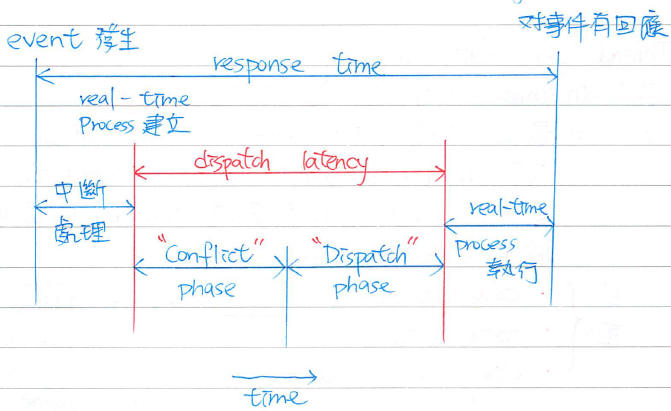
\includegraphics[scale=0.8]{img/real_time_dispatch.png}
                \caption{Dispatch latency on real-time systems.}
                \label{img:real_time_dispatch}
            \end{figure}
        \end{itemize}
    \end{itemize}
\end{theorem}

\begin{theorem}{(80)} Hard real-time system:\begin{itemize}
        \item 討論Synchronous real-time event scheduling,即每隔一段時間發生,需在deadline前完成。
        \item Schedulable判斷:\begin{equation}
            \sum_{i = 1}^{n} \frac{c_i}{p_i} \le 1
        \end{equation} 若符合則schedulable。其中,$n$為事件數目,$c_i$為CPU burst time,$p_i$為period time。
        \item Process meets deadline scheduling algorithms:\begin{itemize}
            \item Rate-Monotonic:\begin{itemize}
                \item Static priority且preemptive。
                \item Period time越小,則priority越高。
                \item Under schedulable,也\textbf{不能}保證所有event皆滿足deadline。
                \item 若其無法滿足deadline,其他static priority scheduling也無法。
            \end{itemize}
            \item EDF (Earliest Deadline First):\begin{itemize}
                \item Dynamic priority且preemptive。
                \item Deadline越小,則priority越高。
                \item Under schedulable,保證所有event皆滿足deadline。
                \item CPU utilization不可能達到$100\%$。
            \end{itemize}
        \end{itemize}
    \end{itemize}
\end{theorem}

\begin{theorem}{(86)} Thread:\begin{itemize}
        \item 又稱Lightweight process。
        \item process是OS分配\textbf{resources}的基本單位,而thread是OS分配\textbf{CPU time}的基本單位。
        \item 同一process之threads共享process的data section (static local and global variables)、heap和code section等,在同一個address可以有多個threads同時執行。
        \item 若一thread被blocked,則CPU可切換給其他thread執行,所以process不會blocked。
        \item Private contents較traditional prcocess少,context switch較快。
        \item 同一process的不同threads可以平行在不同CPUs上執行。
        \item 種類:\begin{itemize}
            \item User-level thread:\begin{itemize}
                \item 由在user site的thread library管理,不需要kernel管理,e.g. POSIX的pthread library,但只是提供規格並沒有實現。
                \item Kernel不知道其存在,因此kernel不干預,導致不同threads\textbf{無法}平行在不同CPUs上執行。
                \item 若user thread發出blocking system call時,則該process也會被blocked,即時該process還有其他available threads。
            \end{itemize}
            \item Kernel-level thread:現行OS皆支持。
        \end{itemize}
        \item pthread library is provided by user-level or kernel-level.
        \item Windows Thread library and Java Thread library are kernel-level threads.
    \end{itemize}
\end{theorem}

\begin{theorem}{(88)} Thread model (user thread-to-kernel thread):\begin{itemize}
        \item Many-to-One model:即user-level thread。
        \item One-to-One model:\begin{itemize}
            \item Not efficient than Many-to-One model.
            \item 若建立過多user thread,kernel overhead過重,performance下降,一般會限制thread數量。
            \item e.g. Linux, family of Windows OS, OSX.
        \end{itemize}
        \item Many-to-Many model:\begin{itemize}
            \item Overhead較One-to-One小,但製作較複雜。
            \item NOT efficient than Many-to-One model.
            \item e.g. Solaris 2,但它是用two-level mapping model製作,同時也允許One-to-One。
        \end{itemize}
    \end{itemize}
\end{theorem}

\begin{theorem}{(90)} Threading issues:\begin{itemize}
        \item \code{fork()} issue:若parent和child thread工作相同,則複製parent process所有threads到child thread;反之,則只複製該thread到child process。
        \item Signal delivery issue: \begin{itemize}
            \item 種類:\begin{itemize}
                \item Synchronous:自作自受,e.g. Divide-by-zero。
                \item Asynchronous:池魚之殃,e.g. aborted by system admin, parent被終止,child也一同被終止。
            \end{itemize}
            \item Signal delivery:\begin{itemize}
                \item Deliver signal to the thread to which the signal applies, e.g. synchronous signal.
                \item Deliver signals to all threads, e.g. user abortion.
                \item Deliver signals to some threads, e.g. kill.
                \item Assign a specific thread to receive all signals for its process, e.g. Solaris 2. 
            \end{itemize}
        \end{itemize}
    \end{itemize}
\end{theorem}

\item \begin{theorem}{(441)} 原始pipeline設計:\begin{itemize}
        \item \code{beq}在$MEM$決定是否要跳。
        \item \code{RegDst}在$EX$。
    \end{itemize}
    \begin{figure}[H]
        \centering
        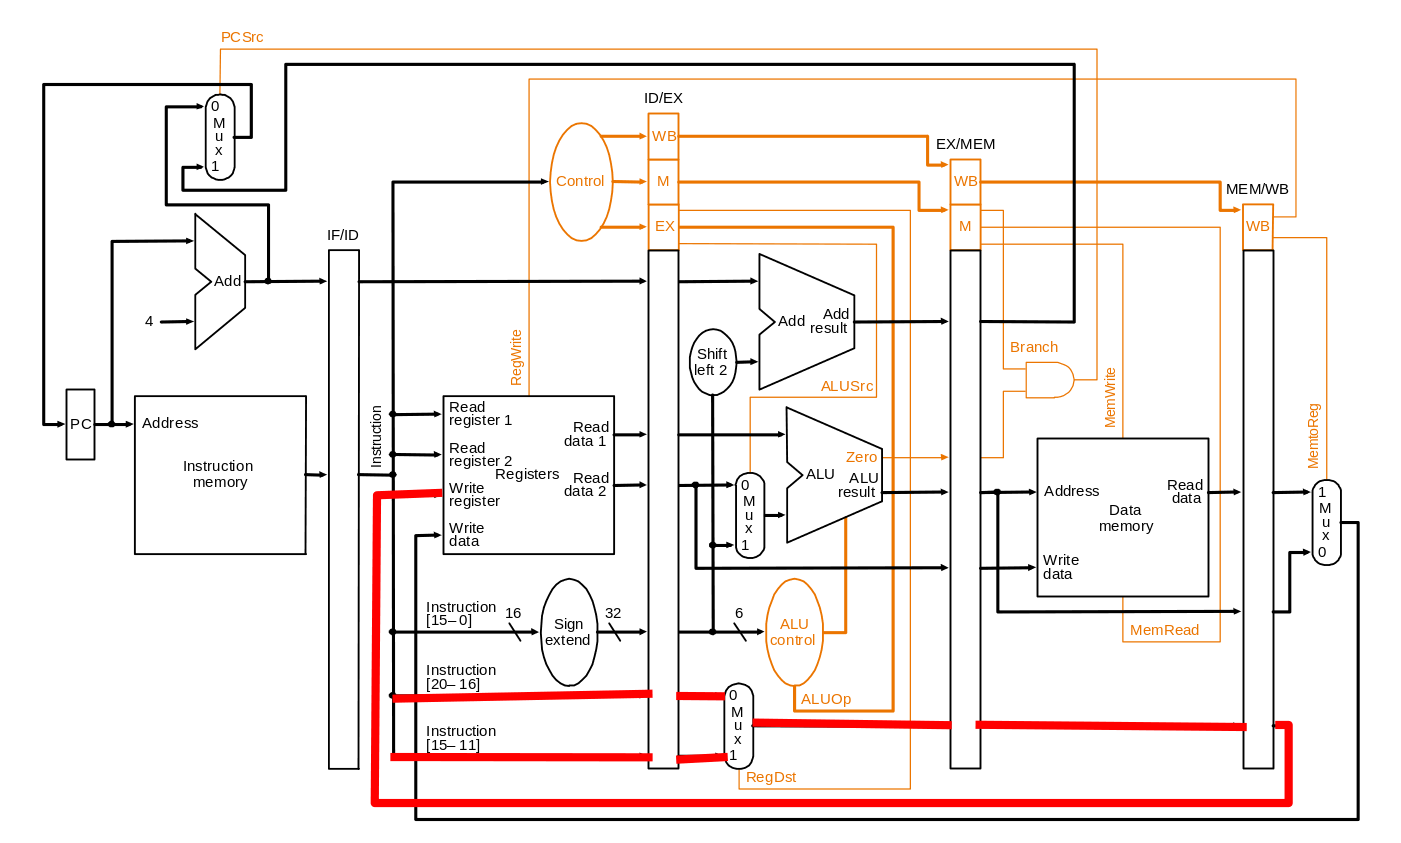
\includegraphics[scale=0.3]{img/pipeline-org.png}
        \caption{Original pipeline.}
        \label{img:pipeline-org}
    \end{figure}
\end{theorem}

\item \begin{theorem}{(450, 455, 457, 458)} Data hazards:\begin{itemize}
        \item Forwarding:Combinational units,放在$EX$因為ALU。
        \begin{lstlisting}[caption={EX hazard.}, captionpos=b, mathescape=true, language={[x86masm]Assembler}, autogobble=true]
            if (EX/MEM.RegWrite $\land$ (EX/MEM.Rd $\neq 0$) $\land$ 
                (EX/MEM.Rd $=$ ID/EX.Rs/Rt))
                ForwardA/B = $10$
        \end{lstlisting}
        \begin{lstlisting}[caption={MEM hazard.}, captionpos=b, mathescape=true, language={[x86masm]Assembler}, autogobble=true]
            if (MEM/WB.RegWrite $\land$ (MEM/WB.Rd $\neq 0$) $\land$ 
                ($\lnot$ EX_hazard) $\land$ (MEM/WB.Rd $=$ ID/EX.Rs/Rt))
                ForwardA/B = $01$
        \end{lstlisting}
        \begin{figure}[H]
            \centering
            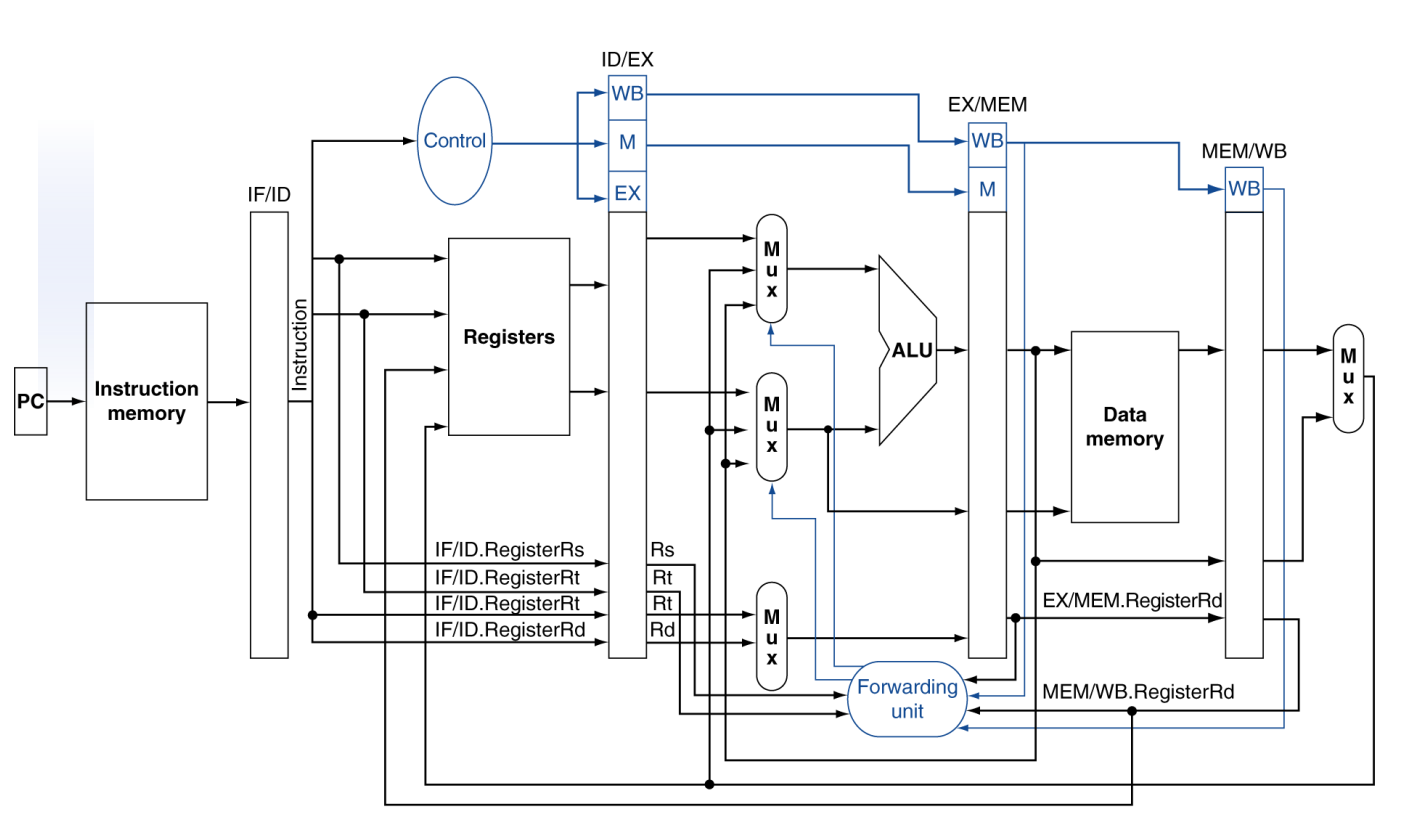
\includegraphics[scale=0.3]{img/pipeline-forward.png}
            \caption{Pipeline with forwarding.}
            \label{img:pipeline-forward}
        \end{figure}
        \item Stall:\code{}
        \begin{lstlisting}[caption={Stall.}, captionpos=b, mathescape=true, language={[x86masm]Assembler}, autogobble=true]
            if (ID/EX.MemRead $\land$ (ID/EX.Rt $=$ IF/ID.Rs/Rt))
                IF/ID.Write := $0$
                PC.Write := $0$
        \end{lstlisting}
        \begin{figure}[H]
            \centering
            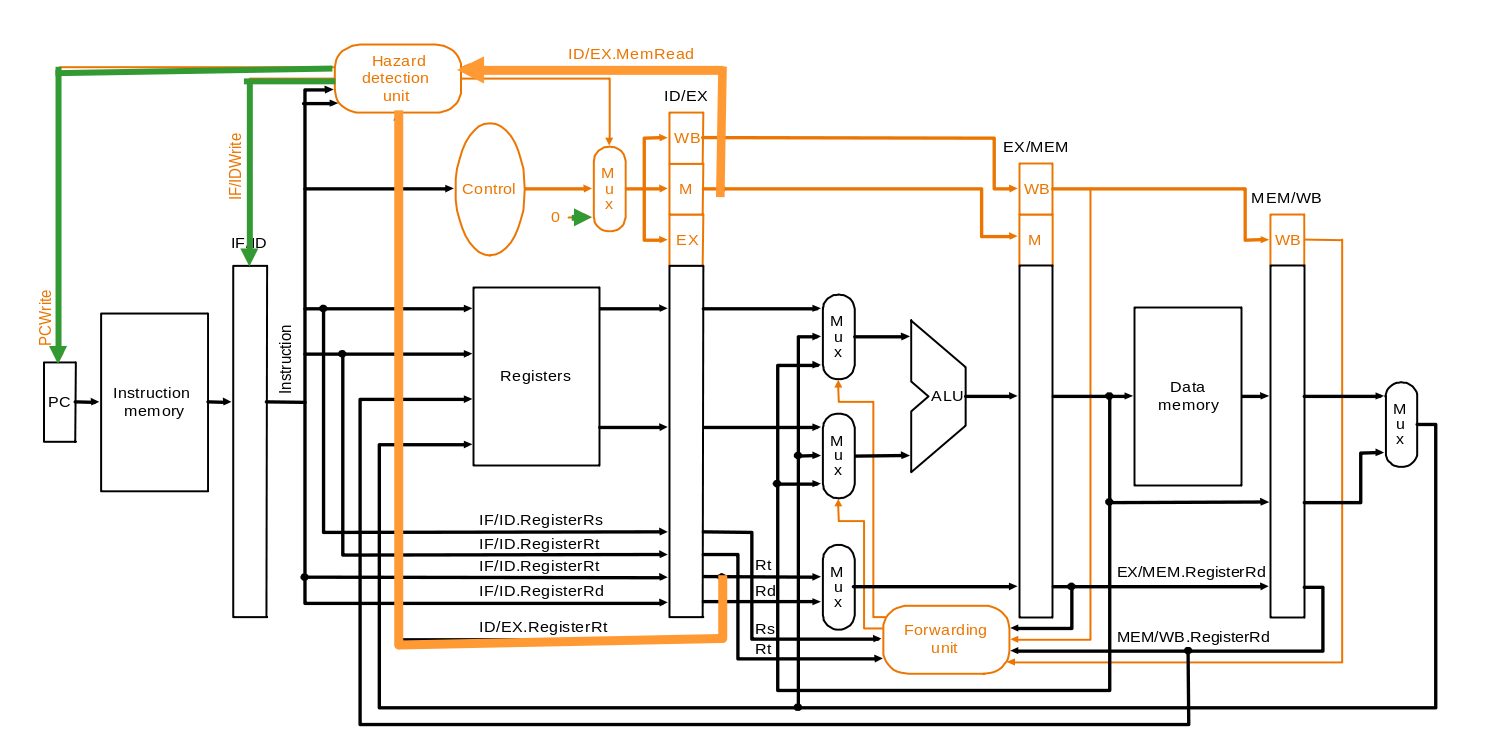
\includegraphics[scale=0.3]{img/pipeline-hazard.png}
            \caption{Pipeline with hazard detection and forwarding units.}
            \label{img:pipeline-hazard}
        \end{figure}
    \end{itemize}
\end{theorem}

\item \begin{theorem}{(478, 487, 494, 559)} Control hazards:\begin{itemize}
        \item 若分支指令與\textbf{前一個ALU指令}或\textbf{前面第二個}\code{lw}有data dependency,必須stall $1$ CC。
        \item 分支指令通過\code{xor}再\code{nor}比較是否相同。
        \begin{figure}[H]
            \centering
            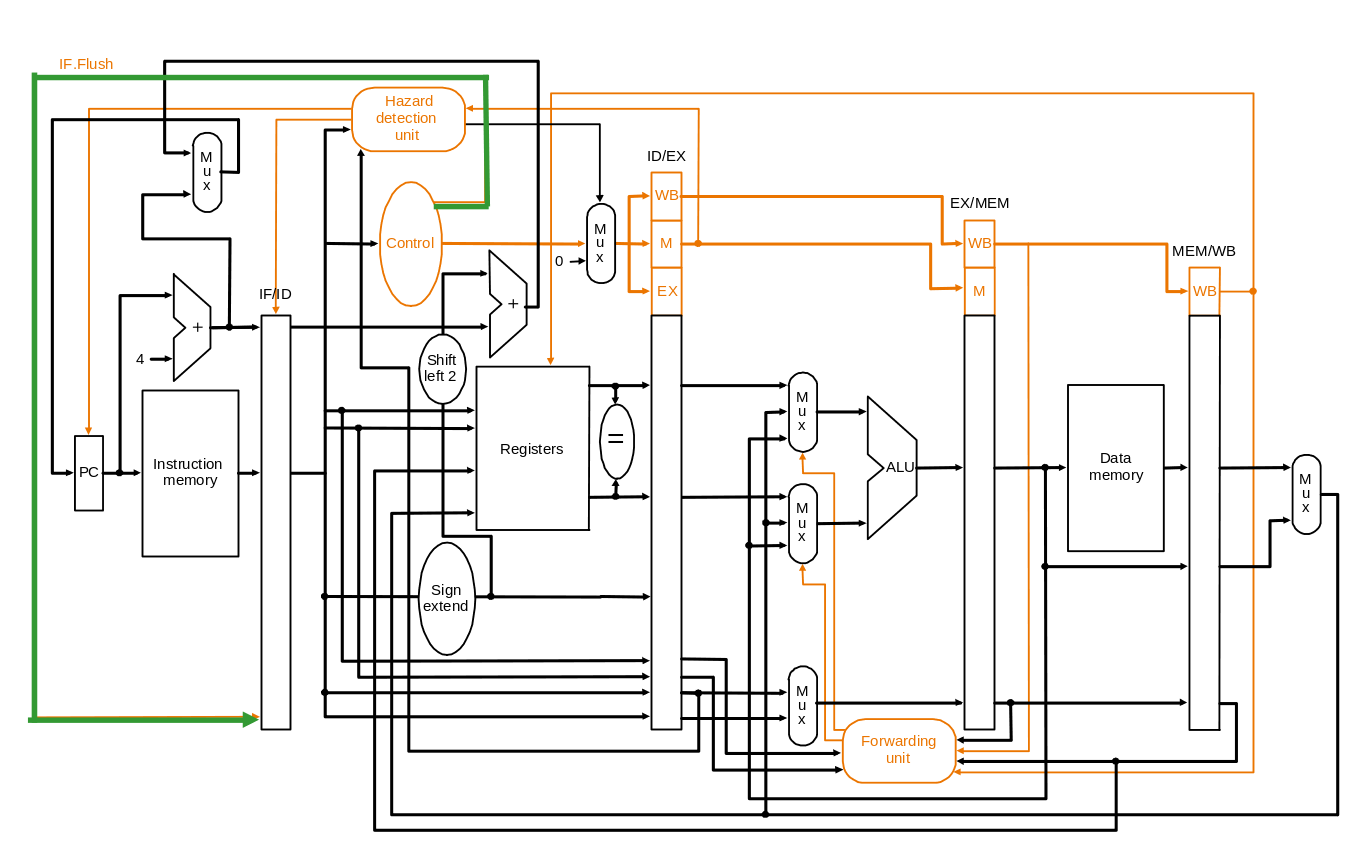
\includegraphics[scale=0.3]{img/pipeline-flush.png}
            \caption{Pipeline with hazard detection, forwarding units and flush.}
            \label{img:pipeline-flush}
        \end{figure}
        \item Delayed branch:\begin{itemize}
            \item NOT suitable for deep pipeline.
            \item From before:最佳方法,不管跳或不跳皆提升。
            \item From target:用於branch發生機率高,有跳才提升。
            \item From fall through:用於branch發生機率低,不跳才提升。
            \begin{figure}[H]
                \centering
                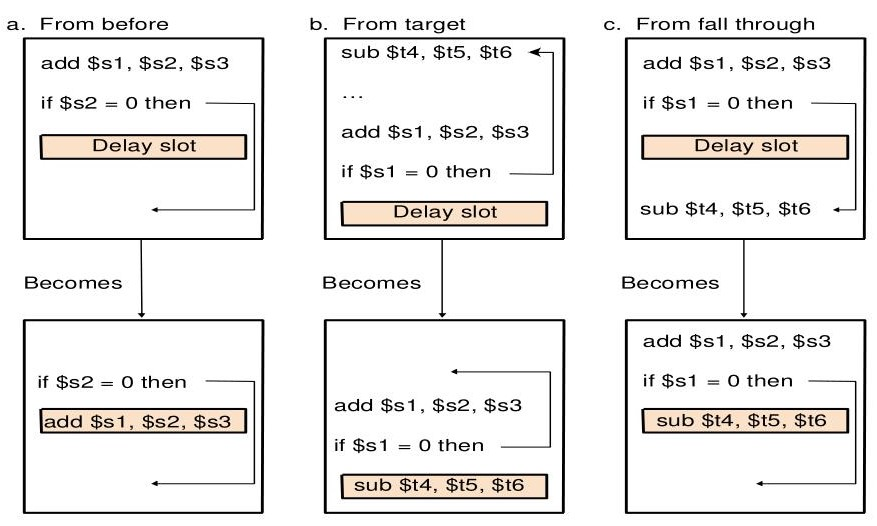
\includegraphics[scale=0.6]{img/delayed-branch.jpg}
                \caption{Example of delayed branch.}
                \label{img:delayed-branch}
            \end{figure}
        \end{itemize}
    \end{itemize}
\end{theorem}

\item \begin{theorem}{(499, 505, 511)} \quad\quad \begin{itemize}
        \item Intel IA-64 (EPIC):\begin{itemize}
            \item 支援利用compiler開發的平行度。
            \item 可以猜測,並利用if-else取代branch。
            \item Registers比MIPS多很多。
            \item Instruction group is a sequence of instructions which does \textbf{NOT} have data dependency and can be executed parallelly.
        \end{itemize}
        \item Speculation錯誤復原:\begin{itemize}
            \item 軟體提供修補程式。
            \item 硬體CPU將猜測結果暫時儲存,若正確,則將猜測結果寫回register或memory,否則flush buffer。
        \end{itemize}
        \begin{table}[H]
            \centering
            \begin{tabular}{|c|c|c|}
                \hline
                \multicolumn{3}{|c|}{Advanced pipeline} \\
                \Xhline{3\arrayrulewidth}
                Technique & Hardware & Software \\
                \Xhline{2\arrayrulewidth}
                Branch prediction & $\surd$ & $\surd$ \\
                \hline
                Speculation & $\surd$ & $\surd$ \\
                \hline
                Intel IA-64 (EPIC) & $\surd$ & $\surd$ \\
                \hline
                Register renaming & $\surd$ & $\surd$ \\
                \hline
                Prediction & & $\surd$ \\
                \hline
            \end{tabular}
        \end{table}
    \end{itemize}
\end{theorem}

\item \begin{theorem}{(515)} MIPS exception handling: \begin{itemize}
        \item Flush the instruction and let all preceding instructions complete if they can.
        \item 利用cause register儲存exception原因。
        \item 將造成exception的instruction memory address存在EPC ($PC + 4$)。
        \item 使用entry point switch to kernel。
        \item Exception handling routine須將$PC - 4$。
    \end{itemize}
\end{theorem}

\item \begin{theorem}{(6.6, 6.7, 6.8, 6.9, 6.10, 6.11, 6.12, 6.16, 6.18)} \quad\quad
    \begin{itemize}
        \item 不含重複\textbf{邊}的路(walk)稱作路線(trail)。封閉路線(trail)稱作迴路(circuit)。
        \item 不含重複\textbf{點}的路(walk)稱作路徑(path)。封閉路徑(path)稱作環路(cycle),其中重複的點不包含起終點,且至少含$3$邊。
        \item 單方向(unilaterally)連通圖:$\forall x, y \in \V, \ x \neq y$,在$x, y$之間存在一條由某一點到另一點的有向路徑。
        \begin{itemize}
            \item 強連通圖必為單方向連通圖,反之不然。
            \item 單方向連同圖必微弱連通圖,反之不然。
        \end{itemize}
        \item 誘導子圖(Induced subgraph):子圖所含原圖之點,皆保留其原有的邊。
        \item 一無向圖,且未必為連通圖,其極大連通誘導子圖稱連通分量圖(Connected component)。
        \item 若在一連通圖上去除一點,使該圖變為不連通圖,則稱該點為切點(cut point或articulation point)。
        \item 若在一連通圖上去除一邊集,使該圖變為不連通圖,且若去除該邊集的真子集不使該圖變為不連通圖,則稱該邊集為切集(cut set)。若切集只含一邊,則稱該邊為切邊(cut edge)或橋(bridge)。
        \item 雙連通圖:無迴圈的連通無向圖且\textbf{不含切點}。
        \item 一無迴圈的連通無向圖,且未必為雙連通圖,其極大雙連通誘導子圖稱雙連通分量圖(Biconnected component)。
        \item 補圖須包含所有點。
        \item 度數為一的點稱懸吊點(pendant)。
        \item 迴圈的度數為$2$。
        \item 一無向圖,所有點的度數皆為$k$,則稱$k$-規則($k$-regular)圖。
        \item 若$G = (\V, \E), \ |\V| = n$,則\begin{equation}
            |\E| \ge \binom{n - 1}{2} + 1
        \end{equation}
        時,$G$為連通圖。
        \item 團(clique):完全子圖,任兩點皆有邊相連。
        \item 獨立集(independent set):補圖的團,任兩點無邊相連。
        \item 支配集(dominating set):支配集中的點與圖上所有點皆有邊相連。
        \item 覆蓋(covering):覆蓋中的點與圖上所有邊相連。
    \end{itemize}
\end{theorem}

\item \begin{theorem}{(6.44, 6.45, 6.47, 6.55)} \quad\quad
    \begin{itemize}
        \item 一簡單無向圖,若所有點的度數至數為$k$,則圖上必含一個長度至少為$k + 1$的環路(cycle)。
        \item 若$G = (\V, \E), \ |\V| \ge 1$為一連通無向圖,則\begin{equation}
            |\E| \ge |\V| - 1
        \end{equation}
        \item 若$A$為一鄰接矩陣,則$A^r$的第$(i, j)$項為$v_i$到$v_j$長度為$r$路的個數。
        \item 一無向圖,為雙分圖$\iff$圖中不含奇數長度的環路。
        \item 若$A$為一鄰接矩陣,則$\frac{1}{6}\tr(A^3)$為圖上三角形個數。
    \end{itemize}
\end{theorem}

\item \begin{theorem}{(6.57, 6.59, 6.60, 6.62)} \quad\quad
    \begin{itemize}
        \item 若存在一路線經過圖中每一\textbf{邊}恰一次稱有尤拉路線(Euler trail)。
        \item 圖中有尤拉迴路$\iff$為連接圖且所有點的度數為偶數。
        \item $K_n$有尤拉迴路$\iff$$n$為奇數。
        \item $K_{m, n}$有尤拉迴路$\iff$$m, n$為偶數。
        \item 圖中有尤拉路線$\iff$為連通圖且圖中恰含$0$個或$2$個點度數為奇數。
        \item 圖中有尤拉迴路$\iff$為強連通圖且所有點的出度數與入度數相同。
    \end{itemize}
\end{theorem}

\item \begin{theorem}{(6.64, 6.68, 6.71, 6.72, 6.73, 6.74, 6.84)} \quad\quad
    \begin{itemize}
        \item 若存在一路境經過圖中每一\textbf{點}恰一次稱有漢米爾頓路徑(Hamiltonian path)。
        \item 漢米爾頓環路必要條件:
        \begin{itemize}
            \item 度數為$2$的點,與其相鄰的邊必在漢米爾頓環路中。
            \item 度數$\ge 2$的點,除了前一條件已知在漢米爾頓環路中的邊之外,其他的邊必不在漢米爾頓環路中。
        \end{itemize}
        \item 有向完全圖必有有向漢米爾頓路徑。
        \item 若$G = (\V, \E), \ |\V| = n \ge 3$為一無迴圈無向圖,
        \begin{itemize}
            \item 若$\deg(x) + \deg(y) \ge n - 1, \ \forall x, y \in \V, x \neq y$,則$G$有漢米爾頓路徑。
            \item 若$\deg(x) + \deg(y) \ge n, \ \forall x, y \in \V, x, y\text{不相鄰}$,則$G$有漢米爾頓環路。
            \item 若$\deg(v) \ge \frac{n - 1}{2}, \ \forall v \in \V$,則$G$有漢米爾頓路徑。
            \item 若$\deg(v) \ge \frac{n}{2}, \ \forall v \in \V$,則$G$有漢米爾頓環路。
        \end{itemize}
        \item $K_n, n \ge 3$必有漢米爾頓環路。
        \item 若一圖有漢米爾頓環路,則該圖中任兩點至少有兩條路徑相連。
        \item 一連通雙分圖,若圖中有漢米爾頓環路,則兩邊的頂點數相同。$K_{m, n}, \ \forall m, n \ge 2$有漢米爾頓環路$\iff$$m = n$。
        \item 一連通雙分圖,若圖中有漢米爾頓路徑,則兩邊的頂點數相差$\le 1$。$K_{m, n}, \ \forall m, n \ge 2$有漢米爾頓路徑$\iff$$|m - n| \le 1$。
        \item $K_n$有$\frac{(n - 1)!}{2}$個相異漢米爾頓環路。
        \item $K_n$,$n$為奇數,有$\le \frac{n - 1}{2}$個\textbf{不共邊}的漢米爾頓環路。
        \item $K_{n, n}$有$\frac{1}{2}n!(n - 1)!$個相異漢米爾頓環路。
        \item 若$G = (\V, \E), \ |\V| = n$,則\begin{equation}
            |\E| \ge \binom{n - 1}{2} + 2
        \end{equation}
        時,$G$有漢米爾頓環路。
    \end{itemize}
\end{theorem}

\item \begin{theorem}{(6.88, 6.90, 6.93, 6.94, 6.97, 6.98)} \quad\quad
    \begin{itemize}
        \item 一無迴圈無向圖,在圖中一邊中加上一頂點,使其變為二邊,稱基本區分(elementary subdivision)。
        \item 二無迴圈無向圖,若二圖同構或皆可由某個圖經由數次基本區分得到,稱二圖同胚(homeomorphic)。
        \item Kuratowski's theorem:平面圖$\iff$\textbf{不}含子圖與$K_5$或$K_{3, 3}$同胚。
        \item 當一個邊在一個區域出現二次,該邊的度數為二。
        \item Euler formula:若$G = (\V, \E), |\V| = v, |\E| = e, r\text{為區域個數}, M\text{為分量圖數}$為平面圖,則$v - e + r = 1 + M$。
        \item 若$G = (\V, \E), |\V| = v, |\E| = e \ge 2, r\text{為區域個數}$為無迴圈簡單\textbf{連通}平面圖,則\begin{itemize}
            \item \begin{equation}
                \frac{3}{2}r \le e \le 3v - 6
            \end{equation}
            \item 若$G$不含任何三角形,則\begin{equation}
                e \le 2v - 4
            \end{equation}
            \item 若每個環路$\ge k \ge 3$邊組成,則\begin{equation}
                e \le \frac{k}{k - 2}(v - 2)
            \end{equation}
        \end{itemize}
        \item 雙分圖不含三角形。
        \item 一無迴圈簡單平面圖必含一個度數$\le 5$的頂點。
    \end{itemize}
\end{theorem}

\item \begin{theorem}{(6.109, 6.110, 6.113, 6.114, 6.115, 6.116)} \quad\quad
    \begin{itemize}
        \item $\chi(K_n) = n$,$\chi(W_n) = 1 + \chi(C_n)$,$\chi(C_n) = \begin{cases}
            2, & n = 2k \\ 3, & n = 2k + 1
        \end{cases}$。
        \item 若$K_n$為一圖$G$的子圖,則$\chi(G) \ge n$。
        \item 雙分圖$\iff$$2$-著色$\iff$圖中不含奇數長的迴圈。
        \item 任意平面圖皆為$4$-著色,反之不然。
        \item 若$G = (\V, \E)$為無向圖,$\lambda$為顏色數,則稱$P(G, \lambda)$為著色多項式,表示至多使用$\lambda$種顏色著色的不同方法數,且$\chi(G) = \min\{\lambda | P(G, \lambda) > 0\}$。\begin{itemize}
            \item $P(G, \lambda)$常數項為$0$。
            \item $P(G, \lambda)$係數和為$0$。
            \item $P(G, \lambda)$最高次項係數為$1$。
        \end{itemize}
        \item 若$G = (\V, \E)$為連通無向圖,$e = \{a, b\} \in \E$,$G \cdot e$為$G - e$中將$a, b$二頂點黏合後的圖,則\begin{equation}
            P(G, \lambda) = P(G - e, \lambda) - P(G \cdot e, \lambda)
        \end{equation}
        \item 若$G = (\V, \E)$為連通無向圖,$e = \{a, b\} \notin \E$,$G \cdot e$為$G + e$中將$a, b$二頂點黏合後的圖,則\begin{equation}
            P(G, \lambda) = P(G + e, \lambda) + P(G \cdot e, \lambda)
        \end{equation}
        \item 若$G = (\V, \E)$為無向圖,且$G_1, G_2$為$G$子圖、$G = G_1 \cup G_2$、$G_1 \cap G_2 = K_n$,則\begin{equation}
            P(G, \lambda) = \frac{P(G_1, \lambda)P(G_2, \lambda)}{\lambda(\lambda - 1)\cdots(\lambda - (n - 1))}
        \end{equation}
    \end{itemize}
\end{theorem}

\subsection{Memory management}

\begin{theorem}{(222)} Binding:\begin{itemize}
        \item 決定在process執行在memory起始address。
        \item 時間點:\begin{itemize}
            \item Compiling time by compiler. 通常只有OS commands採用,e.g. COM file。
            \item Loading/Linking time by linking loader.
            \item Execution time by OS, so called dynamic binding. MMU (Memory Management Unit):Translation from logical (virtual) to physical address.
        \end{itemize}
    \end{itemize}
\end{theorem}

\begin{theorem}{(223)} Dynamic loading:\begin{itemize}
        \item Load-on-call,execution time需要才load。
        \item Process execution time較久,且牽扯到I/O。
        \item 不需要OS協助,programmer責任。
    \end{itemize}
\end{theorem}

\begin{theorem}{(223)} Dynamic linking:\begin{itemize}
        \item Modules code在execution time需要才link。
        \item 節省object code space。
        \item Shared library,助於library更新。
        \item 需要OS協助,因為processes間無法access彼此的memory。
    \end{itemize}
\end{theorem}

\begin{theorem}{(229, 230)} Contiguous allocation:\begin{itemize}
        \item 被占用的space也稱partition,通常是variable,也稱variable partition。Partititon數量也是process數量,即multiprogramming degree。
        \item Process利用linked list管理free memory blocks (holes),稱作Available list (AV-list)。
        \item External fragmentation:\begin{itemize}
            \item Free memory blocks總和夠大,但各自不夠。
            \item Compaction:移動執行中的process,使不連續memory blocks變連續。不易制定optimal policy,且process必須是dynamic binding才行在execution time移動memory blocks。
            \item Page memory management:
        \end{itemize}
        \item Internal fragmentation:配給process的space過多。
    \end{itemize}
\end{theorem}

\begin{theorem}{(242)} Virtual memory:\begin{itemize}
        \item Less I/O time,但總體I/O time上升,因為次數提升。
        \item \begin{equation}
                \text{EMAT} = (1 - p) \times \text{Memory Access time} + p \times \text{Page fault time}
        \end{equation} $p$ is page fault rate.
    \end{itemize}
\end{theorem}

\begin{theorem}{(246)} Page replacement:\begin{itemize}
        \item LRU近似:\begin{itemize}
            \item Second chance (Clock):先用FIFO挑出一個page,若同時reference bit為$0$,則為victim page,但若為$1$,則reset reference bit,loading time改為現在時間,重新FIFO找page。
            \item Enchanced second chance:選擇$<reference, dirty>$最小者,若多個pages相同,則採用FIFO。
        \end{itemize}
        \item 所有replacement algorithms沒有最差,只有最佳。
        \item Belady amonaly:分給process的frames增加,但page fualt rate不降反升。
        \item Stack property:$n$ frames所包含的page set必定是$n + 1$ frames所包含的page set的子集合。且具有stack property的法則,不會發生belady anomaly。只有\textbf{OPT}和\textbf{LRU}有。
        \item Page buffering:\begin{itemize}
            \item Free frames pool:將frames分為\begin{itemize}
                \item Resident frames分配給process。
                \item Free frames pool,OS keep,讓miss pages先行載入,process即可恢復執行,且加入resident frames,完成後再將victim page write back to disk,並歸還free frames pool。
            \end{itemize} 
            \item Keep modification list紀錄dirty bit為$1$的所有page no.,等到OS空閒再將list中的pages write back to disk and reset dirty bits。
        \end{itemize}
    \end{itemize}
\end{theorem}

\begin{theorem}{(253)} Frame allocation:\begin{itemize}
        \item Process可分配frames數量由hardware決定,最多為physical memory size,最少須讓任一machine code完成,即週期中最多可能memory access數量,e.g. $IF$, $MEM$, $WB$共三次。
        \item 解決thrashing:\begin{itemize}
            \item 若已發生,只能降低multiprogramming degree。
            \item 利用page fault frequency control防止thrashing,OS訂定page fault rate合理的上下限,thrashing理當不會發生。若大於上限,應該多分配frames;若小於下限,應該取走一些frames。
        \end{itemize}
        \item Working-set model:\begin{itemize}
            \item 若符合locality,則可降低page fault rate;違反locality:linked list, hashing, binary search, jump, indirect addressing mode。
            \item 可預防thrashing,對於prepaging也有益。
        \end{itemize}
        \item \begin{itemize}
            \item Bigger paging disk沒幫助。
            \item \textbf{Faster paging disk有幫助},因為decrease page fault time。
            \item \textbf{Increase page size有幫助}。
            \item Decrease page size沒幫助。
            \item \textbf{Local repalcement有幫助},因為thrashing不至於擴散。
            \item \textbf{Prepaging有幫助},若猜測夠準,decrease page fault rate。
        \end{itemize}
    \end{itemize}
\end{theorem}

\begin{theorem}{(258)} Page size越小:\begin{itemize}
        \item Page fault rate增加。
        \item Page table size增加。
        \item I/O次數增加。
        \item Internal fragmentation輕微。
        \item I/O transfer time較小。
        \item Locality較佳。
        \item 趨勢:大page size。
    \end{itemize} 
\end{theorem}

\begin{theorem}{(261)} Copy-on-write:\begin{itemize}
        \item \code{fork()} without Copy-on-write:Child and parent processes占用不同空間,且複製parent process content給child process,大幅增加memory space需求,且process creation較慢。
        \item \code{fork()} with Copy-on-write:Child process共享parent process memory space,不allocate new frames,降低memory space需求,且不須複製parent process content,process creation較快,但在write時,
        allocate new frame給child process,並複製內容,修改child process的page table指向new frame,最後才write。
        \item \code{vfork()} (Virtual memory \code{fork()}):Child process共享parent process memory space,不allocate new frames,但不提供Copy-on-write,因此在write時,另一方會受影響。適用於child process create後馬上\code{execlp()},e.g. UNIX shell command interpreter。
    \end{itemize}
\end{theorem}

\end{enumerate}
\endgroup
\bibliographystyle{plain}
\bibliography{content/bibliography}
\addcontentsline{toc}{section}{References}


\end{document}
